% !TEX encoding = UTF-8 Unicode.

% Based on https://github.com/Miracle0565/BUCT-Beamer-Theme

\documentclass[
10pt,
aspectratio=43,
]{beamer}
\setbeamercovered{transparent=10}
\usetheme[
%  showheader,
%  red,
  purple,
%  gray,
%  graytitle,
  colorblocks,
%  noframetitlerule,
]{Verona}

\usepackage[T1]{fontenc}
\usepackage{tikz}
\usepackage[utf8]{inputenc}
\usepackage{lipsum}
%%%%%%%%%%%%%%%%%%%%%%%%%%%%%%%
% Mac上使用如下命令声明隶书字体,windows也有相关方式,大家可自行修改
\providecommand{\lishu}{\CJKfamily{zhli}}
%%%%%%%%%%%%%%%%%%%%%%%%%%%%%%%
\usepackage{tikz}
\usetikzlibrary{fadings}
%
%\setbeamertemplate{sections/subsections in toc}[ball]
\usepackage{xeCJK}
\usepackage{listings}
\usepackage{caption}
\usepackage{subfigure}
\usefonttheme{professionalfonts}
\def\mathfamilydefault{\rmdefault}
\usepackage{amsmath}
\usepackage{multirow}
\usepackage{booktabs}
\usepackage{bm}
\setbeamertemplate{section in toc}{\hspace*{1em}\inserttocsectionnumber.~\inserttocsection\par}
\setbeamertemplate{subsection in toc}{\hspace*{2em}\inserttocsectionnumber.\inserttocsubsectionnumber.~\inserttocsubsection\par}
\setbeamerfont{subsection in toc}{size=\small}
\AtBeginSection[]{%
	\begin{frame}%
		\frametitle{Outline}%
		\textbf{\tableofcontents[currentsection]} %
	\end{frame}%
}

\AtBeginSubsection[]{%
	\begin{frame}%
		\frametitle{Outline}%
		\textbf{\tableofcontents[currentsection, currentsubsection]} %
	\end{frame}%
}

\title{高等数学C}
%\subtitle{A Simple while elegant template}
\author[P.Yu]{余沛}
\mail{peiy\_gzgs@qq.com}
\institute[Guangzhou College of Technology and Business]{Guangzhou College of Technology and Business \\
  广州工商学院}
\date{\today}
\titlegraphic[width=4cm]{logo.png}{}




%%%%%%%%%%%%%%%%%%%%%%%%%%%%%%%%
% ----------- 标题页 ------------
%%%%%%%%%%%%%%%%%%%%%%%%%%%%%%%%



\begin{document}

\maketitle

%%% define code
\defverbatim[colored]\lstI{
	\begin{lstlisting}[language=C++,basicstyle=\ttfamily,keywordstyle=\color{red}]
	int main() {
	// Define variables at the beginning
	// of the block, as in C:
	CStash intStash, stringStash;
	int i;
	char* cp;
	ifstream in;
	string line;
	[...]
	\end{lstlisting}
}
%%%%%%%%%%%%%%%%%%%%%%%%%%%%%%%%
% ----------- FRAME ------------
%%%%%%%%%%%%%%%%%%%%%%%%%%%%%%%%

\section{变量变化问题}
\subsection{速度问题-I} % 匀速运动的情形
\begin{frame}{变量变化问题}{速度问题-I: 匀速运动的情形}
	考虑某物体 $A$ 以速度 $v$ 运动的情形, 记 $t$ 为物体运动的经过时间长度, $s$ 为物体在 $t$ 时刻运动的路程, 我们有
	\[
		s(t) = v\cdot t.
	\]
	对于时刻 $t_1$, $t_2$ 来说, 我们有
	\[
		s(t_2) = v\cdot t_2 = v\cdot t_1 + v\cdot (t_2-t_1) = s(t_1) + v \cdot (t_2-t_1).
	\]
	也就是说
	\[
		s(t_2) - s(t_1) = v \cdot (t_2-t_1), \quad v=\frac{s(t_2)-s(t_1)}{t_2-t_1}.
	\]
\end{frame}

\subsection{速度问题-II} % 匀加速运动的情形

\begin{frame}{变量变化问题}{速度问题-II: 匀加速运动的情形}
	考虑某物体 $A$ 以初速度 $v_0$, 加速度 $a$ 运动的情形, 记 $t$ 为物体运动的经过时间长度, $v(t)$ 为物体在$t$时刻的速度, $s(t)$ 为物体在 $t$ 时刻运动的路程, 我们有
	\[
		v(t) = v_0+a\cdot t.
	\]
	对于时刻 $t_1$, $t_2$ 来说, 我们有
	\[
		v(t_2) = a\cdot t_2 = a\cdot t_1 + a\cdot (t_2-t_1) = v(t_1) + a \cdot (t_2-t_1).
	\]
	也就是说
	\[
		v(t_2) - v(t_1) = a \cdot (t_2-t_1), \quad a=\frac{v(t_2)-v(t_1)}{t_2-t_1}.
	\]
\end{frame}

\begin{frame}{变量变化问题}{速度问题-II: 匀加速运动的情形}
	在前序知识中, 我们知道下式子以及相关的变形,
	\[
		s(t) = v_0\cdot t+ \frac{1}{2}a\cdot t^2
	\]
	那么有
	\begin{align*}
		s(t_2) - s(t_1) &= v_0\cdot (t_2-t_1)+ \frac{1}{2}a\cdot (t_2^2-t_1^2)\\
		&=v_0\cdot(t_2-t_1) + a\cdot(t_2-t_1) \cdot \frac{1}{2}(t_2+t_1),
	\end{align*}
	即
	\begin{align*}
		\frac{s(t_2) - s(t_1)}{t_2-t_1} = v_0 + a\cdot \frac{1}{2}(t_2+t_1).
	\end{align*}
	对比匀速运动的速度定义, 我们可以看到, $t_1\sim t_2$ 期间的平均速度
	\begin{equation*}
		\tilde{v}=\frac{s(t_2) - s(t_1)}{t_2-t_1} = v_0 + a\cdot \frac{1}{2}(t_2+t_1).
	\end{equation*}
	我们考虑速度 $t_2$, $t_1$ 足够接近的情况, $\lim_{(t_2-t_1)\to 0}\tilde{v}=v_0+a\cdot t_1$, 一致?
\end{frame}

\subsection{速度问题-III} % 一般加速运动的情形
\begin{frame}{变量变化问题}{速度问题-II: 匀加速运动的情形}
	\begin{exampleblock}{高超声速飞行器速度问题 \color{blue}(\small{\it 郭建国等, {现代防御技术}, 49(6) 2021.12.)}}
		平飞高超声速飞行器的加速度 $a$ 的简化计算模型为: 
		\begin{align*}
			m\cdot a(t)= \frac{1}{2}\rho(s) v(t)^2 S C_T,
		\end{align*}
		其中, $m$ 是飞行器质量, $v(t)$ 是飞行器速度, $\rho(s)$ 是大气密度, $S$ 是飞行器截面积参考参数, $C_T$ 是油门控制值. 这种问题, 只给出$\rho(s)$, $S$, $C_T$ 和初速度, 如何计算路程和速度?	
	\end{exampleblock}
	思路: 极限, 逐步求解.
\end{frame}


\subsection{函数的切线问题-I} % 二次函数的切线问题
\subsection{函数的切线问题-II} % 一般函数的切线问题
\subsection{抽象-一般变量变化问题}


\section{Basics}
\subsection{块}
\begin{frame}[c]{Blocks}
	
The blocks are shown below
这是一个block
\begin{block}{Regular Block}
	Content of a regular block
\end{block}

\begin{exampleblock}{Example Block}
	Content of an example block
\end{exampleblock}

\begin{alertblock}{Alert block}
	Content of an alert block
\end{alertblock}

\end{frame}	

\subsection{Enumerate \& Overlays}

\begin{frame}[c]{Enumerate \& Overlays}
	
{\large An Example of \texttt{enumerate}}
	\begin{enumerate}[<+->]
		\item First item
		\item Second item
		\item Third item
	\end{enumerate}
\vfill
{\large An Example of \texttt{itemize}}	
	\begin{itemize}[<+->]
	\item First item
	\item Second item
	\item Third item
	\end{itemize}
\end{frame}	

\subsection{Two columns}
\begin{frame}[c]{Two columns}
	
\begin{columns}[onlytextwidth]
	\column{0.4\textwidth}
	Content for column one
	\begin{equation}
	E = mc^2
	\end{equation}
	\column{0.4\textwidth}	
	Content for column two
	\begin{equation}
	F=ma
	\end{equation}
\end{columns}
\end{frame}	

\begin{frame}{分栏:左图右字或者左字右图}
\begin{columns}
	\column{0.5\textwidth}
		\begin{figure}
		\centering
		% Requires \usepackage{graphicx}
		\includegraphics[width=5cm]{logo}
		\caption{分栏示意图}
	\end{figure}
	\column{0.55\textwidth}
	\small
	这里输入文字
\end{columns}
\end{frame}


\subsection{Figures}
\begin{frame}[c]{Figures}
	\begin{figure}
		\centering
		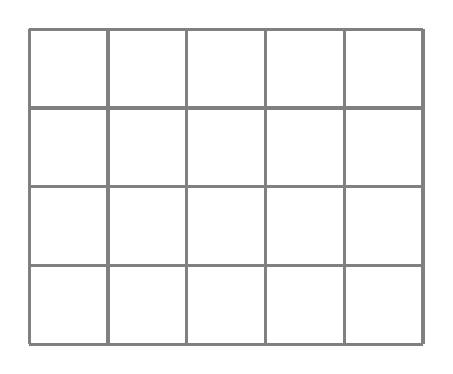
\begin{tikzpicture}
		\draw [help lines,very thick] (0,0) grid (5,4);
		\end{tikzpicture}
		\caption{Credits to Ti\textit{k}Z}
	\end{figure}
\end{frame}	

\begin{frame}{Figures}
怎么插入多张图片:
\begin{figure}[h]
    \centering
    \subfigure[校徽1]{
    \includegraphics[scale=0.022]{logo.png}
    }
    \subfigure[校徽2]{
    \includegraphics[scale=0.022]{logo.png}
    }
    \subfigure[校徽3]{
    \includegraphics[scale=0.022]{logo.png}
    }
    \subfigure[校徽4]{
    \includegraphics[scale=0.022]{logo.png}
    }
    \caption{demo}
\end{figure}
\end{frame}

\subsection{Code Demo}
\begin{frame}{A Listings Demo}{C++}
	\lstI
\end{frame}

\section{References}

\begin{frame}{BibTex使用}
    这里引用文献\cite{9492070}。
\end{frame}

\begin{frame}{References}
\bibliographystyle{abbrv}     %论文引用格式
\bibliography{References}


\end{frame}
% Thank you page
\beamertemplateshadingbackground{structure.fg!90}{structure.fg}
\begin{frame}[plain]
	\vfill
	\centering
	{
		\centering \Huge \color{white} Thank you for your attention!\\[10pt]Questions?
	}
	\vfill
\end{frame}


\end{document}


